\documentclass[10pt]{article}

\usepackage[margin=0.6in]{geometry}
\usepackage[T1]{fontenc}
\usepackage{lmodern}
\usepackage{xcolor}
\usepackage{booktabs}
\usepackage{array}
\usepackage{graphicx}
\usepackage{enumitem}
\usepackage{titlesec}
\usepackage{listings}
\usepackage[hidelinks]{hyperref}
\usepackage{natbib}

\setlist{noitemsep, topsep=2pt, partopsep=0pt, parsep=0pt, leftmargin=1.4em}

\titlespacing*{\section}{0pt}{6pt plus 1pt minus 1pt}{2pt}
\titlespacing*{\subsection}{0pt}{4pt plus 1pt minus 1pt}{2pt}
\titleformat{\section}{\normalfont\large\bfseries}{\thesection}{0.6em}{}
\titleformat{\subsection}{\normalfont\bfseries}{\thesubsection}{0.6em}{}

\linespread{0.95}\selectfont
\setlength{\parskip}{1.5pt}
\sloppy
\setlength{\parindent}{0pt}

\lstset{
  basicstyle=\ttfamily\scriptsize,
  breaklines=true,
  columns=fullflexible,
  frame=single,
  framesep=2pt,
  xleftmargin=2pt,
  xrightmargin=2pt,
  aboveskip=2pt,
  belowskip=2pt
}

% Greppable placeholder for any not-yet-measured value.
\newcommand{\TODO}[1]{\textcolor{red}{\textbf{[TODO: #1]}}}

\pagestyle{empty}

\begin{document}

{\Large \bfseries Agentic Computational Reproducibility of Published Research on CORE-Bench}\\[2pt]
{\large CSE598 (Agentic AI) --- Capstone Project Proposal}

\vspace{2pt}
\renewcommand{\arraystretch}{1.0}
\begin{tabular}{@{}p{0.30\linewidth}p{0.66\linewidth}@{}}
\toprule
\textbf{Student name} & Jason Lunder \\
\textbf{Project title} & Agentic Computational Reproducibility of Published Research on CORE-Bench \\
\textbf{Repository / notebook link} & \url{https://github.com/jlunder00/repro-agent} \\
\textbf{Configuration location} & \texttt{examples/} and \texttt{.env.example} \\
\bottomrule
\end{tabular}

\section{Problem Definition}
Published code capsules often fail to run after release because of dependency rot, undocumented environments, or ambiguous run instructions. \textbf{User:} a researcher, reviewer, or student who holds a paper and its capsule, must confirm that the reported numbers come out of the code, and has no working environment for it. \textbf{Input:} a code capsule (source plus README and/or Dockerfile) and questions about its reported results; some questions ask about values shown in the capsule's figures. \textbf{Output:} a \texttt{report.json} mapping each question to an answer. \textbf{Success:} every answer falls inside the benchmark's 95\% prediction interval built from three ground-truth runs (exact match when those runs agree). \textbf{Failure:} any wrong answer, a crash, or no file produced.

\section{Motivation and Project Scope}
We target CORE-Bench \citep{siegel2024corebench,corebenchgithub}: 270 tasks from 90 papers (Python and R), 45 train / 45 test papers, each at three tiers: \emph{easy} (a successful run's output is given, execution forbidden), \emph{medium} (Dockerfile plus README), and \emph{hard} (README only; the agent installs dependencies and infers commands).

\textbf{Why agentic.} The hard tier requires acting on an environment and observing state that is unavailable up front: tracebacks, file layout, version incompatibilities. The \S4 trace shows two failures, the second visible only after the first fix; a single call cannot see them and a rule-based installer cannot read them. Structurally this is SWE-bench for environments: the agent changes the environment, not the code, and the target is a number, not a passing test.

\textbf{Claim.} CORE-Agent is AutoGPT in continuous mode with a \$4 budget; it already observes failures and re-plans, so ``add an iterative loop'' is not a contribution. The capstone adds two mechanisms CORE-Agent lacks: (a) \emph{date-aware dependency resolution}: each \texttt{pip install} is resolved to the newest release predating the capsule's publication date (available via \texttt{capsule\_doi}), which fixes the \texttt{xlrd==1.2.0} class of failure before the traceback rather than after retries; (b) \emph{base-image selection as an agent action} instead of a fixed per-language lookup. Ablation: the same loop with and without these components, at equal dollar cost.

\textbf{Scope IN:} all 90 capsules (45 train, 45 test), Python and R, at the easy and hard tiers; written and figure questions, with figures passed to the model as images. GPU-flagged capsules are run on CPU. \textbf{Scope OUT:} the medium tier (needs Docker-in-Docker), GPU execution, and repeated runs per task. \textbf{Feasibility:} the sandbox, grader, and single-pass pipeline exist, and one full sweep of 90 capsules at both tiers cost \$2.66 and 41 minutes of wall time; the resolver is one PyPI lookup per package and image selection is one sandbox parameter.

\section{Runnable Baseline}
A single-pass, no-retry pipeline using \texttt{claude-sonnet-5} through \texttt{litellm} and Docker: (1) fetch the capsule, (2) read the README, (3) one LLM call proposing install and run commands, (4) execute once in a base image chosen by capsule language (\texttt{python:3.11-slim} for Python, \texttt{r-base:4.4.1} for R; a fixed lookup, not a decision), (5) one LLM call extracting answers from the run output, the result files, and up to six of the capsule's figures attached as images, (6) write \texttt{report.json}, (7) score with the vendored official grader. Each stage records success or failure, so a failed task is attributed to plan, execute, or extract.

\textbf{Files:} \texttt{run\_baseline.py} (CLI); \texttt{src/repro\_agent/dataset.py} (task list, filters), \texttt{capsules.py} (download, cache, tier preparation), \texttt{llm.py} (litellm wrapper, image input, cost tracking), \texttt{sandbox.py} (Docker execution), \texttt{baseline.py} (pipeline), \texttt{scoring.py} (vendored official grader).

\textbf{Why a reasonable start:} it is the floor. The experimental control for the capstone is the capstone loop at one iteration, sharing prompts and environment with the treatment arm, so the ablation isolates the two mechanisms rather than two codebases.

\section{Test Case and Baseline Output}
Example: \texttt{capsule-9052293} (1.0\,MB), an ANP-TOPSIS tourism model. \textbf{Input:} the capsule plus \emph{``Report the closeness coefficient for location L1.''} \textbf{Expected output:} \texttt{report.json} containing \texttt{0.844703753651819}; all three ground-truth runs are identical, so an exact match is required.

\begin{center}
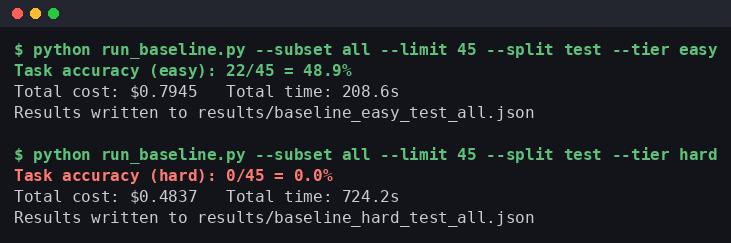
\includegraphics[width=0.68\linewidth]{figures/baseline_output.png}\\[1pt]
{\small Figure 1: Baseline output on the test split at both tiers. The train split gives 21/45 easy and 0/45 hard.}
\end{center}

\textbf{Easy (90 capsules, figures attached):} 43/90 tasks (47.8\%); 63/98 written questions (64.3\%), 38/83 vision questions (45.8\%), 101/181 overall (55.8\%); 152 images sent; \$1.61 total, \$0.0178 per task. By split and language: test Python 15/22, test R 7/23, train Python 17/27, train R 4/18. Without images the model scored 7/54 on vision questions. \textbf{Hard (90 capsules):} 0/90 tasks, 0/181 questions; the execute stage succeeded 0/90 in every split and language; \$1.04 total, 22.0\,s per task. No run was aborted: extraction ran on the failed output and returned \texttt{null}. For \texttt{capsule-9052293} the plan was \texttt{pip install openpyxl pandas \&\& cd code \&\& python script.py}. Manual tracing shows two sequential fixes, the second visible only after the first: (i) \texttt{ModuleNotFoundError: xlrd}; (ii) \texttt{xlrd}~2.x dropped \texttt{.xlsx} support, so \texttt{xlrd==1.2.0} is required --- an older release of the package just installed. With both, the capsule reproduces \texttt{0.844703753651819} exactly.

\section{Reproducibility and Run Instructions}
Python 3.10+. \texttt{pip install -r requirements.txt} (\texttt{litellm} is pinned \texttt{<1.60}; later releases fail on Python 3.10). Copy \texttt{.env.example} to \texttt{.env}, set \texttt{ANTHROPIC\_API\_KEY} or \texttt{OPENAI\_API\_KEY}, then \texttt{export \$(grep -v \textquotesingle\textasciicircum\#\textquotesingle{} .env | xargs)}. Task metadata and prompts are in \texttt{examples/}. Single capsule, easy: \texttt{python run\_baseline.py -{}-capsule capsule-9052293 -{}-tier easy}. Full split: \texttt{python run\_baseline.py -{}-subset all -{}-limit 45 -{}-split test -{}-tier easy}; repeat with \texttt{-{}-split train} and \texttt{-{}-tier hard}. The hard tier needs a running Docker daemon. Capsules are downloaded into \texttt{capsules/} on first use; output goes to \texttt{results/baseline\_<tier>\_<split>.json} (override with \texttt{-{}-out}); the committed runs are \texttt{results/baseline\_<tier>\_<split>\_all.json}. \texttt{-{}-list} prints the selection without a key. Medium tier: not implemented.

\section{Initial Evaluation Plan}
Development uses the train split (45 tasks per tier); evaluation uses the test split (45 tasks per tier). Primary metric: official task accuracy. Secondary metrics: written-question and vision-question accuracy, since task accuracy is all-or-nothing. Also recorded: execution success rate, cost, latency, failure stage. Each arm runs at least 3 times per task because the model is sampled without a fixed temperature; results are mean and range at matched cost. Improvement means the arm with the resolver and image selection beats the arm without them at equal cost, same model, task set, and grader. The published numbers below are context only: different model, year, and harness; they are not a like-for-like baseline.

\begin{center}\scriptsize
\begin{tabular}{@{}llccc@{}}
\toprule
Agent & Model & Easy & Medium & Hard \\
\midrule
CORE-Agent & GPT-4o & 60.00\% & 57.78\% & 21.48\% \\
AutoGPT    & GPT-4o & 35.56\% & 37.78\% & 6.67\%  \\
\midrule
This baseline (test split, 45 tasks) & claude-sonnet-5 & 48.9\% & --- & 0.0\% \\
\bottomrule
\end{tabular}\\[1pt]
{\scriptsize Rows 1--2: \citet{siegel2024corebench}, Table 5 (pass@1, test split, 45 tasks/tier). Row 3: \S4, one run, not comparable.}
\end{center}

\section{Limitations and Next Steps}
\emph{Figure cap}: at most 6 figures are attached per capsule, chosen by sorted filename; 13 capsules have more, so a question about a figure outside that set stays unanswerable. \emph{Result truncation}: result files are concatenated in directory order up to a character budget, so an answer late in a long log can be cut off. \emph{Single run}: one run per task with no fixed temperature, so repeated runs are needed before any comparison of arms. \emph{All-or-nothing scoring}: per-question accuracy is reported alongside task accuracy. \emph{Base image}: the per-language lookup is fixed; R hard-tier execution succeeded 0/41 even with the correct interpreter, so image choice must become a recorded variable in both arms. \textbf{Needed:} API and container budget for repeated sweeps (90 tasks $\times$ 2 arms $\times$ 3 runs, up to 900\,s each) and a Docker host. \textbf{Next:} the loop; the date-aware resolver; image selection; a verification run for extracted values; repeated runs.

{\scriptsize
\setlength{\bibsep}{0pt}
\bibliographystyle{plainnat}
\bibliography{references}
}

\end{document}
